\documentclass{article}
\usepackage[T1]{fontenc}
\usepackage[utf8]{inputenc}
\usepackage{lmodern}
\usepackage{amsmath}
\usepackage{sansmath}
\AtBeginDocument{\sansmath}
\renewcommand{\familydefault}{\sfdefault}
\usepackage[paperwidth=19cm,paperheight=14cm,margin=0.4cm]{geometry}
\usepackage{graphicx}
\usepackage{tikz}
\usetikzlibrary{positioning,fit,calc,arrows.meta,backgrounds,decorations.pathreplacing}
\pagestyle{empty}
\setlength{\parindent}{0pt}
\graphicspath{{img/}}

\definecolor{ink}{HTML}{0A0A0A}
\definecolor{muted}{HTML}{6A6A69}
\definecolor{line}{HTML}{BDBDBA}
\definecolor{red}{HTML}{E03A3A}
\definecolor{blue}{HTML}{2E6FE0}
\definecolor{yellow}{HTML}{D9A11A}
\definecolor{green}{HTML}{23A06A}
\definecolor{model}{HTML}{8C8C8A}

\tikzset{
  every picture/.style={font=\sffamily\small, line cap=round, line join=round},
  flecha/.style={-{Stealth[length=2.3mm,width=1.7mm]}, line width=0.7pt, draw=ink},
  grupo/.style={draw=#1, dash pattern=on 3pt off 2pt, line width=0.8pt, rounded corners=2pt, inner sep=6pt},
  titulo/.style={font=\sffamily\small\bfseries, text=#1, anchor=south west, inner sep=1pt},
  foto/.style={inner sep=0pt, outer sep=0pt, draw=ink, line width=0.5pt},
  caja/.style={draw=ink, line width=0.5pt, fill=#1, text=white, font=\sffamily\scriptsize\bfseries,
    text width=3.75cm, minimum height=0.46cm, align=center, inner sep=1.5pt},
  nota/.style={font=\sffamily\scriptsize, text=muted, align=center, inner sep=1pt},
  etapa/.style={font=\sffamily\footnotesize\bfseries, text=ink, align=center, inner sep=1pt},
  paso/.style={draw=ink, line width=0.5pt, fill=#1, text=ink, font=\sffamily\scriptsize, align=center,
    inner sep=3pt, minimum height=0.95cm, text width=2.35cm},
  paso/.default=white,
  grupofondo/.style={draw=#1, line width=0.8pt, fill=#1!6, rounded corners=3pt, inner sep=7pt},
  llave/.style={decorate, decoration={brace, mirror, amplitude=5pt, raise=2pt}, line width=0.7pt, draw=#1},
  llavetexto/.style={font=\sffamily\small\bfseries, text=#1, align=center},
}

\begin{document}
\begin{tikzpicture}

\node[foto] (in) at (0, -0.1) {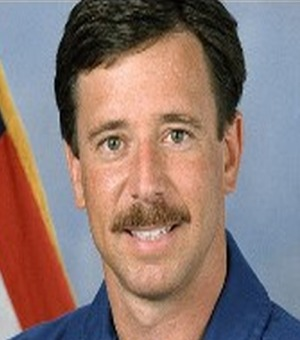
\includegraphics[width=1.7cm]{foto.jpg}};
\node[nota, below=3pt of in] {Foto o cámara};

\node[foto] (pts) at (2.75, 1.05) {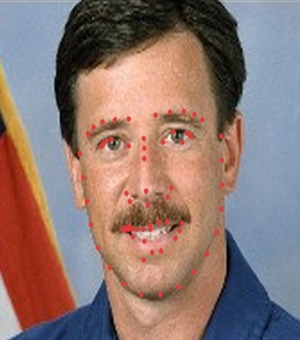
\includegraphics[width=1.45cm]{puntos.jpg}};
\node[nota, below=2pt of pts] (ptslabel) {478 $\rightarrow$ 68 puntos};
\node[foto] (seg) at (2.75, -1.35) {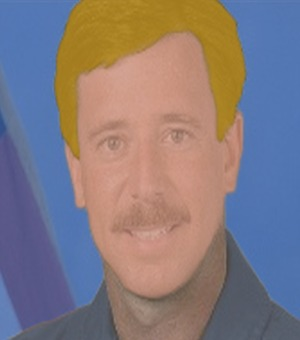
\includegraphics[width=1.45cm]{segmentacion.jpg}};
\node[nota, below=2pt of seg] (seglabel) {pelo, piel y fondo};
\node[grupo=model, fit=(pts)(ptslabel)(seg)(seglabel)] (g1) {};
\node[titulo=muted] at (g1.north west) {Modelos};

\node[foto] (mesh) at (5.65, 1.05) {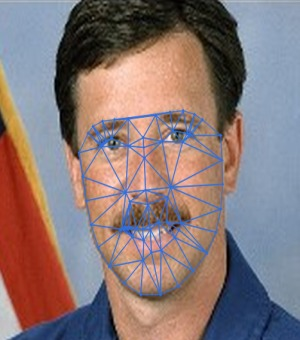
\includegraphics[width=1.45cm]{malla.jpg}};
\node[nota, below=2pt of mesh] (meshlabel) {Delaunay (Fortune)};
\node[foto] (frame) at (5.65, -1.35) {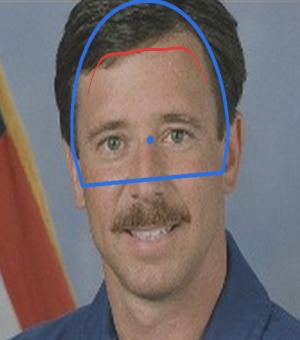
\includegraphics[width=1.45cm]{marco.jpg}};
\node[nota, below=2pt of frame] (framelabel) {marco de la cabeza};
\node[grupo=blue, fit=(mesh)(meshlabel)(frame)(framelabel)] (g2) {};
\node[titulo=blue] at (g2.north west) {Geometría};

\foreach \name/\text/\tono [count=\i] in {
  barba/Barba: warp por triángulo/red,
  tinte/Tinte en CIELAB/red,
  corte/Corte: pull-push y Lambert/red,
  forma/Forma de cara: malla 3D/red,
  vivo/En vivo: Verlet y PBD/red,
  espejo/Espejo 3D: EWA en WebGL2/blue,
  peluca/Peluca 3D: envolvente visual/blue,
  gauss/Gaussianas 2D: Adam/yellow,
  juego/Contrarreloj: cápsula/yellow} {
  \node[caja=\tono, anchor=west] (t\name) at (8.15, {2.82 - 0.58 * \i}) {\text};
}
\node[grupo=red, fit=(tbarba)(tjuego)] (g3) {};
\node[titulo=red] at (g3.north west) {Algoritmos de cada herramienta};

\node[foto] (o1) at (13.55, 0.78) {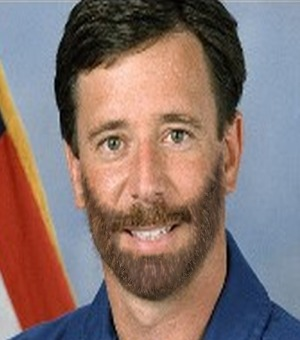
\includegraphics[width=1.2cm]{barba.jpg}};
\node[foto] (o2) at (14.85, 0.78) {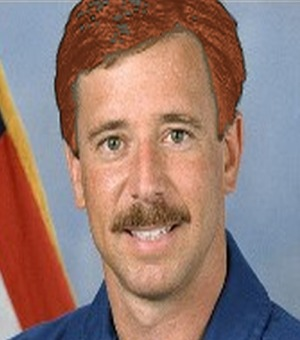
\includegraphics[width=1.2cm]{tinte.jpg}};
\node[foto] (o3) at (13.55, -0.92) {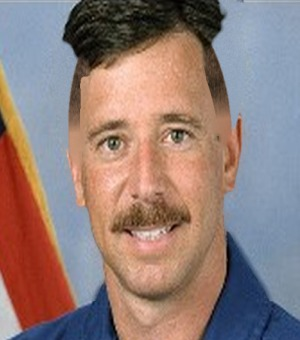
\includegraphics[width=1.2cm]{corte.jpg}};
\node[foto] (o4) at (14.85, -0.92) {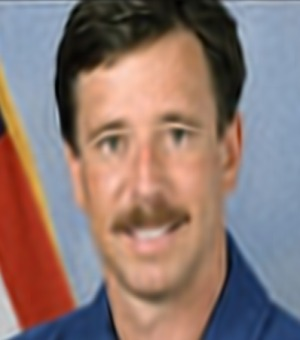
\includegraphics[width=1.2cm]{gaussianas.jpg}};
\node[nota, below=2pt of o3.south east] (olabel) {imagen o gaussianas 3D};
\node[grupo=green, fit=(o1)(o2)(o3)(o4)(olabel)] (g4) {};
\node[titulo=green] at (g4.north west) {Resultado};

\coordinate (mid) at (0, -0.1);
\draw[flecha] (in.east) -- (g1.west |- mid);
\draw[flecha] (g1.east |- mid) -- (g2.west |- mid);
\coordinate (fan) at ($(g2.east |- mid) + (0.3, 0)$);
\draw[line width=0.7pt, ink] (g2.east |- mid) -- (fan);
\foreach \name in {barba, tinte, corte, forma, vivo, espejo, peluca, gauss, juego} {
  \draw[flecha, line width=0.5pt] (fan) to[out=0, in=180, looseness=0.9] (t\name.west);
}
\draw[flecha] (g3.east |- mid) -- (g4.west |- mid);

\coordinate (base) at ($(g3.south) + (0, -0.06)$);
\draw[llave=muted] (g1.west |- base) -- (g1.east |- base)
  node[midway, below=9pt, llavetexto=muted] {Preentrenados:\\solo ubican};
\draw[llave=ink] (g2.west |- base) -- (g3.east |- base)
  node[midway, below=9pt, llavetexto=ink] {Implementado por el equipo};
\draw[llave=green] (g4.west |- base) -- (g4.east |- base)
  node[midway, below=9pt, llavetexto=green] {Salida};

\end{tikzpicture}
\end{document}
